\
%-------------------------------------------------------------------------------
\section{Case Studies}
%-------------------------------------------------------------------------------
\label{sec:hotcrp_example}

\begin{table}[t!]
    \centering
    \footnotesize
    \begin{tabular}{@{}cccc@{}}
        \textbf{Application} & \textbf{\#Object} & \textbf{Schema} &
        \textbf{Disguise} \\
        \textbf{Disguise} & \textbf{Types} & \textbf{LoC} & \textbf{LoC} \\
    \midrule
    \lrtbf & 19 & 318 & 100 \\
    \hrtbf & 25 & 352 & 142 \\
    \hrtbfplus & 25 & 352 & 255 \\
    \hconfanon & 25 & 352 & 232 \\
\end{tabular}
    \caption{Data disguise specifications for Lobsters and HotCRP have similar complexity to
    a relational schema.
}
\label{tab:loc}
\end{table}

%
We evaluate the ease of writing single disguises by writing disguises for GDPR deletion in
Lobsters~\cite{lobsters}, an open-source news feed application, and HotCRP~\cite{hotcrp}.
%
We consider four disguises: \lrtbf and \hrtbf implement the current account
deletion policies in the two applications~\cite{lobsters:privacy, hotcrp:privacy}.
%
\hrtbfplus specifies a HotCRP account deletion policy that balances useful data retention with
data deletion for privacy (\S\ref{design:eg}).
%
Finally, \hconfanon specifies the conference anonymization disguise for HotCRP.

\paragraph{Complexity.}
%
We would hope that writing disguises involves similar labor and difficulty as writing
relational schemas.
%
In particular, a developer should write a disguise only once.
%
Because disguises specify a set number of transformations for each object type,
disguise complexity is limited by the number of object types and relations in the
application schema.
%
Table~\ref{tab:loc} shows that the disguise specification for our applications is indeed
comparable in size to the applications' schemas.
%

\paragraph{Performance.}
\label{sec:perf}

\begin{figure}[t!]
    \centerline{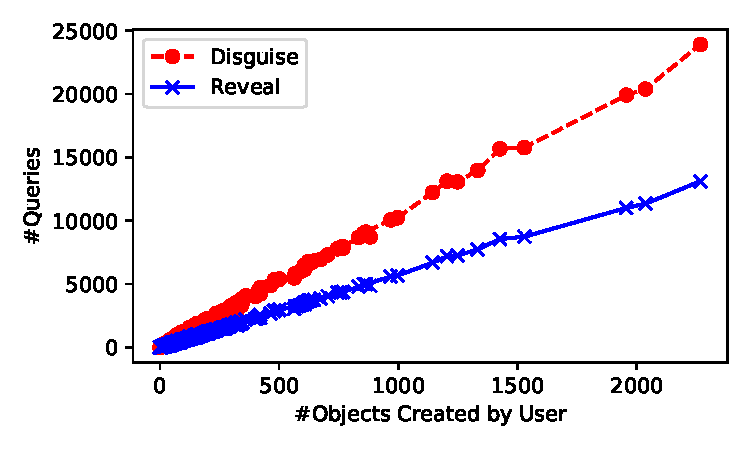
\includegraphics[width=.5\textwidth]{img/perf}}
    \vspace{-\baselineskip}
    \caption{Number of queries required by \lrtbf to disguise and reveal a target user, depending on the number of
    objects created by the user.}
    \label{fig:latencies}
    \vspace{-\baselineskip}
\end{figure}

Our experience implementing \sys exposed the challenging performance implications of both efficiently
executing normal application queries, and achieving low-latency disguise operation. The right
balance depends on the rate of disguising, which may range from rare (as in today's applications)
to quite frequent (in a privacy-supporting world where users freely disguise and reveal themselves,
or where data automatically ages out).

%
When executing a disguise such as user account deletion, \sys may generate as many guises as there are
objects referencing the user, each requiring one or more SQL queries to create. \sys must also
log all updates in the vault, and potentially read and reverse prior vault entries.
%
Figure~\ref{fig:latencies} shows the number of queries run when applying and reversing
\lrtbf on an object graph with 3K users and 80K total user contributions, with no prior
disguises having been applied.
%
The overhead increases linearly with the number of objects created by the target user.  \sys
currently performs transformation queries sequentially; some batching and parallelization is
possible and could improve this performance.
%
The reverse transformation (reveal) starts with the complete data and batches by table.
%
\sys currently runs a disguise in one large SQL transaction, impacting the performance of any other
application queries during disguise execution.

%
Our results indicate the need for privacy-aware database designs, which spread the cost of
disguising across normal execution.
%
One possibility keeps a ``shadow'' copy of the database that reflects the disguised state, with
guises already created and modified.
%
Pre-created guises are hidden by transparently exposing materialized views (MV) to the
application.
%
Disguising then exposes the shadow copy in the MV, and removes disguised objects.
%
This achieves good read performance---queries read from MVs instead of the database---albeit
at the cost of space overhead.
%
However, normal execution write queries must potentially update multiple guises in the
shadow copy, and pre-created guises consume space during normal execution, even if disguises
are never applied.
%
Other possibilities include making disguises eventually consistent; updating the shadow copy
asynchronously; and caching disguises for target objects disguised most often.
